\chapter{Sprint 3}
This chapter covers the development process during the 3rd sprint. The 3rd sprint covers the the implementation of the needed database features for getting a functioning search engine. 


The overall goal for the Knox project during this sprint was to get the search engine to work. To accomplish this goal the product owner specified a list of expectation that when completed would fufill a minimal viable product. The specified list is outlined below.
\begin{itemize}
	\item It should be possible to make searches in all the available databases.
	\item It should be possible to make searches using keywords in all the available data.
	\item It should be possible to make searches in all Nordjyske articles from 2017-2021
	\item It should be possible to make searches in all the Grundfos manuals, barring those that have shown to be problematic during processing.
	\item The UI should minimally be able to display a link to the given article but preferably display the title and text.
\end{itemize}

With the overall goal for the sprint outlined, a granulated sprint goal could be made that accounts for the focus of our scrum group.

\section{Sprint Planning}
\subsection{Knox Goal}
The overall goal for the Knox project during this sprint was to get the search engine to work. To accomplish this goal the product owner specified a list of expectation that when completed would fufill a minimal viable product. The specified list is outlined in figure X.
\begin{itemize}
	\item It should be possible to make searches in all the available databases.
	\item It should be possible to make searches using keywords in all the available data.
	\item It should be possible to make searches in all Nordjyske articles from 2017-2021
	\item It should be possible to make searches in all the Grundfos manuals, barring those that have shown to be problematic during processing.
	\item The UI should minimally be able to display a link to the given article but preferably display the title and text.
\end{itemize}

With the overall goal for the sprint contained in figure x, a granulated sprint goal could be made that accounts for the focus of our scrum group.


\textbf{Sprint goal}
As noted in the preceding sprint, the codebase that was inherited from the previous iteration was deemed problematic and costly to maintain. Therefore our sprint goal for this iteration was based on updating the codebase to better comply with the requirements for the Knox goal.


Based on this observation as well as the aforementioned requirements, our sprint goal was as follows:


\textit{Make the minimally required amount of API endpoints available to satisfy the requirements for the search engine, and create the necessary documentation.}


\textbf{Backlog \& Increments}
The sprint goal could then be granulated into subtasks. With the tasks granulated, a session of scrum poker was held in order to evulate the time requirement of each task. Lastly the tasks were categorized by their priority and focus point and divided into three different sprint increments: Wordcount API, Write Report, Wiki Documentation. 


%%Remember to add an estimate to Write report and wiki update
\begin{table}[]
\begin{tabular}{|l|l|l|ll}
\cline{1-3}
Estimate & Increments                         & Tasks                         &  &  \\ \cline{1-3}
82       & \multicolumn{1}{c|}{Wordcount API} & CRUD operations on controller &  &  \\ \cline{1-3}
X        & Write Report                       & Document the process          &  &  \\ \cline{1-3}
X        & Wiki Update                        & Feature documentation         &  &  \\ \cline{1-3}
\end{tabular}
\end{table}





%\subsection{Sprint goal}
%The sprint goal for this group
%How does our sprint goal help with the overall sprint goal
%The purpose and priority for each increment
%Show the available backlog

\section{Increment 1.}
With the aforementioned tasks in mind, we will now move on to describing the first increment of this sprint.

We start by outlining the different database frameworks considered for the project.
Afterwards, we discuss which framework was chosen and why.


\subsection{CRUD}

As outlined in the planning for this sprint, the main focus of this sprint was to implement API end-points for the database.
As we already had a working database, the goal of this increment was to write a CRUD API in C\# such that the other layers could use to access the database via HTTP requests.
The CRUD operations we implemented are based on requests from the other layers, and what they thought they needed to retrieve from the database.
To implement this, we split the CRUD operations into three different Routes handling different aspects of the database. The routes are called: WordCount, WordRatio and Schema. Each route has its own endpoints and can access different tables in the database. The API has been split into three routes that each cover a section of the database. Wordcount is for inserting articles into the database, WordRatio is used as an absbraction over the WordRatio table in the database, and the Schema route is used to add JSON Schemas to the database.

The pipeline for the API is outlined in figure \ref{Node02Sprint3}.

\begin{figure}[h]
    \centering
    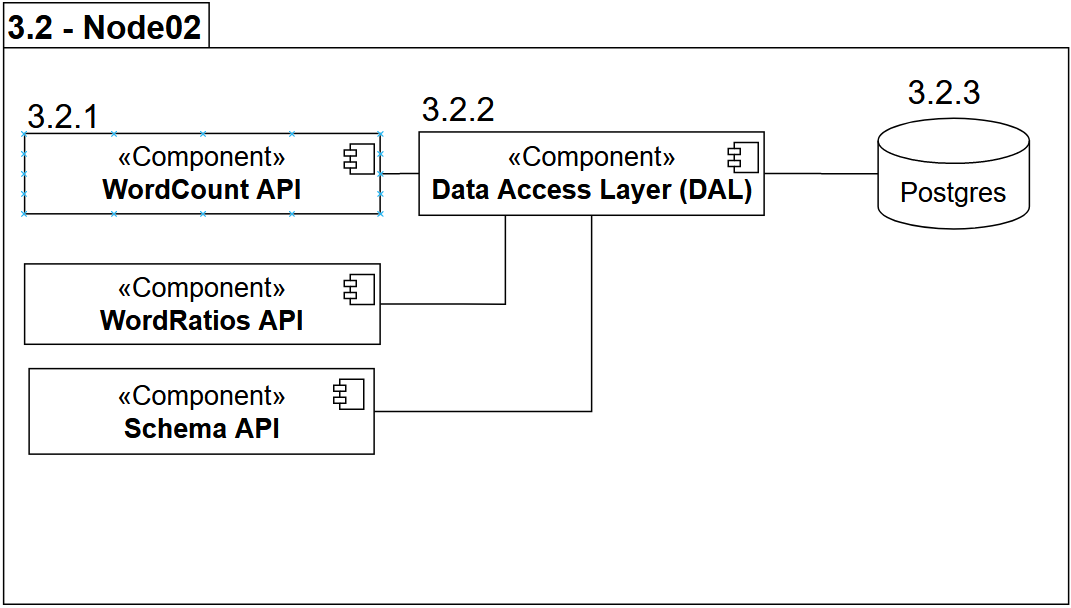
\includegraphics[width=\linewidth]{Images/Node02Sprint3.PNG}
    \caption{Node02 server pipeline in sprint 3.}
    \label{Node02Sprint3}
\end{figure}

\subsubsection{WordCount}

The first route we created was the WordCount route. It is used by the knowledge layer to insert information about an article into the database. It is also used by the functionality layer to find the filepath of an article.

In the controller we implemented 2 methods, a \texttt{GET} and a \texttt{POST} method.
\begin{table}[h]
    \begin{tabular}{|llll|}
    \hline
    \multicolumn{4}{|c|}{\textbf{WordCount}}                                                                                 \\ \hline
    \multicolumn{1}{|l|}{Name}                 & \multicolumn{1}{l|}{Method} & \multicolumn{1}{l|}{Input}       & Response on success       \\ \hline
    \multicolumn{1}{|l|}{\texttt{GetFilepath}} & \multicolumn{1}{l|}{GET}    & \multicolumn{1}{l|}{Integer}     & Article        \\ \hline
    \multicolumn{1}{|l|}{\texttt{Post}}        & \multicolumn{1}{l|}{POST}   & \multicolumn{1}{l|}{JSON Object} & Status message \\ \hline
    \end{tabular}
    \end{table}

The \texttt{GET} method called \texttt{GetFilepath}, takes a integer "id" as an argument and finds an article in the database with the given "id" and returns the articles filePath as a JsonResult if it exists, otherwise an error is sent back.


In WordCount, we also implemented a \texttt{POST} method called \texttt{Post} which takes a JSON object from the HTTP body as a parameter which should correspond to an array of articles. 
The JSON object should be valid according to a JSONschema on the database, which determines the required format of the of the JSON object and the fields needed. If the JSON object does not fit the schema, an error message is sent back. 
The articles are then checked for duplicate data on the database, if there is any it is removed and a message is added to the response that the article already exists. The remaining articles can then be inserted into the database, and a status message is returned with the potential duplicate article names. 
 
\subsubsection{WordRatio}
The WordRatio route is used by the functionality layer to fetch specific data from the database.
As the WordRatio table is a view, it cannot be used to store new data. 
The primary purpose of WordRatio is to check how many times a given word occurs in an article.
WordRatio consists of one \texttt{GET} method with an optional parameter. 
\begin{table}[h]
    \begin{tabular}{|llll|}
    \hline
    \multicolumn{4}{|c|}{\textbf{WordRatio}}                                                                                                                                           \\ \hline
        \multicolumn{1}{|l|}{Name} &
        \multicolumn{1}{l|}{Method} &
        \multicolumn{1}{l|}{Input} &
        Reponse on success \\ 
    \hline
        \multicolumn{1}{|l|}{\texttt{GetMatches}} &
        \multicolumn{1}{l|}{GET} &
        \multicolumn{1}{l|}{terms (string[]), sources (string[])} &
        WordRatio for all articles from source with term \\
    \hline
        \multicolumn{1}{|l|}{\texttt{GetMatches}} &
        \multicolumn{1}{l|}{GET} &
        \multicolumn{1}{l|}{terms (string [])} &
        WordRatio for all articles with term \\
    \hline
    \end{tabular}
\end{table}

The \texttt{GetMatches} method is used to query one or more specific words on the WordRatio table.
One may provide one or more sources in which to search for the specified words.
If no sources are provided, the database searches for the given words in all sources.
The Rows of the table matching the terms and sources.

\subsubsection{Schema}
The last route we implemented in this iteration is the Schema route which is used to post and retrieve a JSON schema from the database. These are later used to verify JSON objects as input on other endpoints. 
This schema consists of two \texttt{GET} methods and a single \texttt{POST} method.
By creating a route for fetching the validation schemas, we enable easy validation and a common understanding of the structure of input data from the knowledge layer.
\begin{table}[h]
    \begin{tabular}{|llll|}
    \hline
    \multicolumn{4}{|c|}{\textbf{Schema}}                                                                                                     \\ \hline
    \multicolumn{1}{|l|}{Name}                     & \multicolumn{1}{l|}{Method} & \multicolumn{1}{l|}{Input}               & Response on success \\ \hline
    \multicolumn{1}{|l|}{\texttt{GetSchema}}       & \multicolumn{1}{l|}{GET}    & \multicolumn{1}{l|}{SchemaName (string)} & JSON Schema         \\ \hline
    \multicolumn{1}{|l|}{\texttt{GetAllSchemas}}   & \multicolumn{1}{l|}{GET}    & \multicolumn{1}{l|}{None}                & All JSON Schemas    \\ \hline
    \multicolumn{1}{|l|}{\texttt{PostJSONSchemas}} & \multicolumn{1}{l|}{POST}   & \multicolumn{1}{l|}{JSON Schema}         & Status message      \\ \hline
    \end{tabular}
\end{table}

The first \texttt{GET} method is called GetSchema which takes a SchemaName as its input and returns a JSON Schema. 

The second \texttt{GET} method is called GetAllSchemas which takes no input and returns all stored JSON schemas. 

The last method is a \texttt{POST} method called PostJSONSchema and takes a JSON Schema as its input and inserts it into the database.
The body of the post request must consist of two fields - the schema name, which is its primary key in the database, and the schema content itself. Before the schema is inserted in the database it is checked if it is a duplicate, if that is the case an error message will be sent in response.
A schema gets stored in the database in the format known as \texttt{jsonb} or JSON binary which is a built-in type provided by \postgres{}.
This format is used to store a JSON object as binary which uses much less space than a \texttt{varchar} or regular JSON type would.
Even though \postgres{} may not be the most efficient DBMS for storing JSON data, it is sufficient for this use case, as posting and fetching Schemas will not be done often. 
\subsection{Docker}
Docker is an open source containerization platform that allows for a simplification of deliveries in distributed applications through the usage of containers.\cite{Container_Docker} 
Before giving a more detailed description of Docker, an overview of what a container is and how it is used is needed. 


Containers were originally developed to solve the issue where a program may work on one system but encounter problems when moved to a different one. 
Using containers allows developers to package their code together with its required dependencies. 
Moving around a prepackaged application with all its dependencies ensures that the software is going to run the same regardless of the infrastructure in place.\cite{Container_Docker} 


A container image is a lightweight version encapsulating everything needed to run that application. These images are then turned into containers at runtime. 
This is made possible by the build process isolation and virtualization capabilities in the Linux kernel. 
These capabilities allow for multiple application components to share the resources of single host operating system, 
in much the same way a hypervisor allows multiple virtual machines to share the same hardware resources of a single computer.\cite{Container_Docker}


Using Docker rather than a virtual machine provides the following advantages:

\begin{itemize}
    \item Lighter weight
    \item Resource efficiency
    \item Improved developer productivity
\end{itemize}

Docker itself is then used to enhance these native Linux features allowing us to automate container creation and easily move the containers between environments.\cite{Docker_IBM}
\subsection{Continuous Integration and Delivery}
In our work, we have used both Continuous Integration (CI) and Continuous Delivery (CD).
For CI, we have used GitHub with GitHub Actions. We have created a GitHub Actions workflow that
runs the tests in our project; and another one that tests the code quality. These checks run every time commits are made towards the main branch. This ensures that we keep that branch production-ready
at all times.

For CD, we have implemented an automatic deployment system that deploys the code to the production server.
We start the workflow by tagging the commit with the version number. Once we push the tag, a GitHub Actions
workflow is triggered that deploys the code to the production server.
To facilitate the deployment, we containerized our software. The Action workflow starts by building the
Docker image, which is pushed to the GitHub Package Repository. On the production server, we have a Docker 
container watching for new releases. When a new release is pushed, the container pulls the new image and
deploys it.


\section{Review}
The goal for this sprint can be seen in section \ref{ssec:sprint3Goal}. We were to implement part of the Knox Search Engine MVP, which meant that we were to facilitate data access and storage.

\subsubsection{What has been accomplished?}
This sprint, we have implemented operations for the WordCount API. This was done in close collaboration with the neighboring layers. 
Besides this, we also wrote documentation for the relevant implementation details. A full overview of what was done can be seen below.

\begin{itemize}
    \item \texttt{GET} \& \texttt{POST} API endpoints for the WordCount database.
    \item WordRatio response objects for endpoints, rather than previous layers directly querying the view.
    \item API for JSON schemas used for validating data sent to the API.
    \item API project and database containerized.
    \item Development and production environment set up and configured for rapid development \& deployment.
    \item Implemented CI/CD using Docker and GitHub Actions.
    \item Restructured database using a code-first approach.
    \item Repository-unit of work pattern has been implemented to promote encapsulation and separation of concerns.
    \item Wiki restructuring and documentation of configuration and API.
\end{itemize}

While we did manage to implement most of what was requested of us, we did not document this to the extent that our Definition of Done requires. 
We have decided to carry over these tasks to the next sprint, prioritizing them first. In the sprint retrospective, we will discuss why we did not accomplish everything we wanted to, and what we are doing about it.

Towards the end of this sprint, we demonstrated an end-to-end test to the \knox{} product owner. The pipeline seemed to work well, and we were able to get the product to work as expected. This was later confirmed by the PO. 
Six days after the end-to-end test, an API endpoint stopped working due to heavy memory load. We pushed a hotfix to fix this shortly after.

\subsubsection{What has changed in the environment?}
For this sprint, the primary focus has been to implement the Knox Search Engine. As such, all other groups have had the same focus, and therefore they have not requested anything from the database layer yet. 
We expect to see a lot of changes to the database layer in the next sprint, as some groups have mentioned that they would like to store different types of data next sprint.
A full overview of what has changed can be seen below.

\begin{itemize}
    \item The structure of the objects' sent from the below layer have changed: a 'publication' field has been introduced in the schema defining the object.
    \item We found out that the Knox Product Owner will not be creating a new backlog with tasks for us to solve, but that we should rather create meaningful tasks ourselves.
    \item We have made other groups realize that creating server-users, database schemas based on their use-cases, and similar task are their responsibility.
\end{itemize}

\subsubsection{What next?}
As mentioned before, we were asked to suggest possible next steps for our share of the Knox project. The below list encapsulates our suggestions---some of which are based upon requests from other groups.

\begin{itemize}
    \item At the Scrum of Scrum retrospect, many groups told that they want to work with knowledge graphs. Therefore, we should prepare for tasks regarding the RDF database.
    \item We should be prepared to provide assistance with the WordCount database endpoints. This included minor changes and new endpoint implementation.
    \item Potentially, we could benchmark database technologies for the Knox project, to find a good option for the Knox use-case.
\end{itemize}
\section{Retrospective}

\subsection{Reflection on the sprint}
All features planned during the sprint planning phase was implemented by the end of the sprint, but we did not document the code as well as we had initially planned. 
This clashes with our Definition Of Done, which means we did not fully reach the goal of this sprint. We have attached our Definition of Done in section \ref{sec:definitionOfDone}.

We planned out the implementation to a certain degree, but used a non-optimal format for the tasks, which led to confusion down the line. Namely, we should have described what the task encapsulated more than giving it a simple name--like 'POST'. 

We also did not use user-stories, which contributed to the confusion, as they would have otherwise provided a certain context for the tasks.

The remaining tasks were lackluster and-or nonexistent, which led to trouble doing structured writing, as we had to figure out what should be written every time we wanted to write.
    
To some extent, this was caused by conflicting information given by various sources. We also received a lot of 'urgent, but not important' tasks from other groups, which we had to react to immediately.
    
Due to the above, there were times when individual members did not exactly know what we had finished nor what other members were working on. Tasks were added almost daily, continuously changing the scope of the sprint.
As such, we did not hit our original point-estimate---it became completely irrelevant due to the rapid changes in scope.

\subsection{What we learned}\label{Whatwelearnedsprint3}
We learned that we had to be more vigilant about narrowing the scope of our tasks. 
This was especially true when working on the API's where we initially thought that we should develop full CRUD capabilities, but it turned out that only some of the capabilities were necessary. 
From this we gathered that we should use some agile method to better our understanding of the needs of different layers.

We should not change response object structure after it has been deployed---we could solve this by implementing classes that represent the response objects, instead of sending domain models. 

Intergroup communication was a big part of the sprint, as we had to work with other groups to get the right information. 
Working together while testing gave great insight into the needs of the other groups, and we were able to implement the desired features much quicker.

As the semester courses taught us more about agile methods, we found that we did a few things in a non-conventional way. Planning poker was a great way to get a sense of the scope of the sprint, but we should have used a more structured way to do it. 
Instead of the way we played in during sprint planning, we will make the following optimizations:
Each participant has a set of cards with numbers on. These numbers represent the relative sizing of a task, which is why it is common to use the Fibonacci sequence, where the numbers are well spread out.
Each round begins with the Product Owner reading a user story, which is then discussed. Then, each participant selects a card with their estimate of the task. Once every participant has selected a card, the cards are turned over. If everyone is within two cards of each other, the average of the numbers on the cards is taken as the user story estimate. If that is not the case, the outliers will discuss, and a new round commences.
This is done until there are no more user stories left\cite{sutherlandScrumArtDoing2014}.


We also learned that doing velocity analysis is a great way to know if team productivity is actually improving, which should be a result of us implementing optimizations and removing impediments.
Tasks should also not be marked as complete before they have been shipped to production, as per Scrum convention---a task is not done before it is delivered\cite{sutherlandScrumArtDoing2014}.

\subsection{How we can improve in the next sprint}

\subsubsection{Start doing}

\begin{itemize}
    \item Create user stories based on input from stakeholders
    \item Specification of the data in the database---this should be given to the other groups so fewer issues regarding CRUD operations occur
    \item Update the Kanban board frequently, so group members always are updated
    \item Change planning poker strategy:
    \subitem If everyone is within two cards of each other, just average the sum of your cards.
    \subitem If people are more than three cards apart, the high and low cards talk about why they think what they do.
    \subitem Don't estimate in hours, estimate in 'work' (relative size).
    \item Velocity analysis
    \item Component diagram versioning---we want to show the progress!
    \item Tasks are not done before they are released. We will make a lane on our Kanban board as a landing for them while they wait for deployment.
    \item Sprints changed to 2-week duration. 4 weeks is too long.
\end{itemize}

Having concluded the sprint, we will proceed to the next sprint. As mentioned earlier, we will start by documenting what we did not document during this sprint. 
Other tasks will be defined during the sprint planning process, which will be discussed in the next chapter.

